\section{Application Scenarios}
\label{sec:caseStudy}
% \shusen{A full case study that driven by the visualization task and the question associated with them}
%In this section, we discuss application scenarios, in which the domain experts utilize the 
To better illustrate how the proposed perturbation-driven exploration tool helps researchers interpret the neural network model, we present five application scenarios gathered by the domain experts who integrated the proposed tool into their model analysis workflow.
%Here 

\begin{figure}[htbp]
\centering
\vspace{-2mm}
 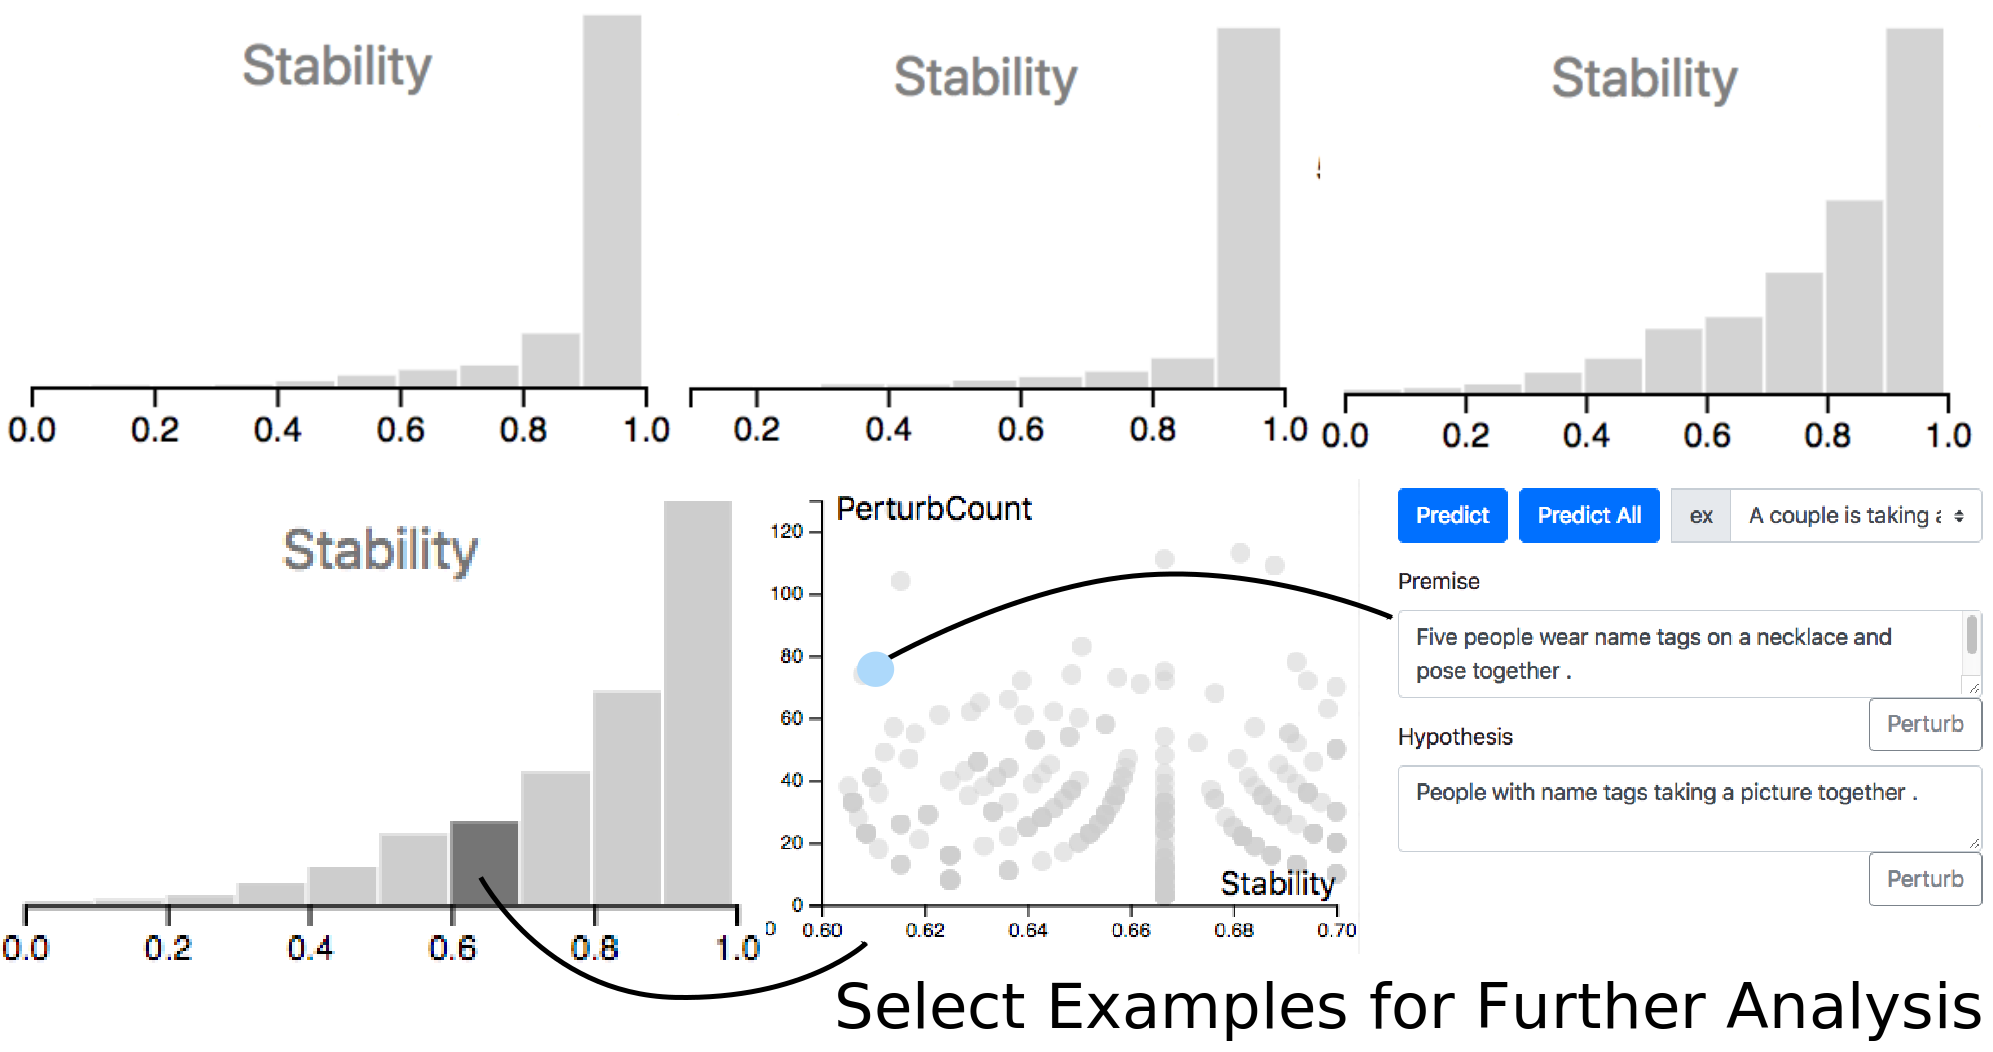
\includegraphics[width=1.0\linewidth]{predictStability}
 \caption{
Prediction stability assessment. In (a)(b)(c), we estimate the overall prediction stability (regarding synonymous perturbation) for each type prediction over the entire development set (100k examples). The user can drill down to individual examples by filtering via the histogram and scatterplot (see Fig.~\ref{fig:summaryView}) for a case by case exploration, as illustrated in (d)(e). For highly unstable outliers, we often observe the prediction of the original sentences near the decision boundary (e.g., the yellow circle in (f) corresponds to a entailment prediction that is very close to neural), however, some predictions, such as the one illustrated in (d) can alter the prediction quite drastically with minor perturbation (illustrated in $d_1$, where the word ``heap'' is replace by ``pile'' in the hypothesis sentence).
%
}
\label{fig:predictStability}
\end{figure}

\subsection{Scenario 1: Assess the Model Prediction Stability}
The robustness of the prediction is often the information the researchers wish they know, yet hard measure easily.
Utilize the automated system input sentence perturbation to assess the overall stability of the prediction.
As illustrated in Fig.~\ref{fig:predictStability}, we estimate the overall prediction stability (regarding synonymous perturbation) for each type prediction over the entire development set (100k examples). The user can drill down to individual examples by filtering via the histogram and scatterplot (see Fig.~\ref{fig:summaryView}) for a case by case exploration, as illustrated in (d)(e). For highly unstable outliers, we often observe the prediction of the original sentences near the decision boundary (e.g., the yellow circle in (f) corresponds to a entailment prediction that is very close to neural), however, some predictions, such as the one illustrated in (d) can alter the prediction quite drastically with minor perturbation (illustrated in $d_1$, where the word ``heap'' is replace by ``pile'' in the hypothesis sentence


\subsection{Scenario 2: Examine the Decision Making Process}
\begin{itemize}
\item What alignment the prediction looks for attention alignment
\item 
\end{itemize}

%Hypothesizing
Interpreting how the model arrive at a prediction is one of the most important goal for the expert driven exploratory analysis.
%

 first step  only essential for evaluating the model performance but also necessary for hypothesizing improvement strategies.
%
The three stages (encoder, attention, classifier) of the model work in synergy to produce the correct prediction.

\begin{figure*}[t]
\centering
\vspace{-2mm}
 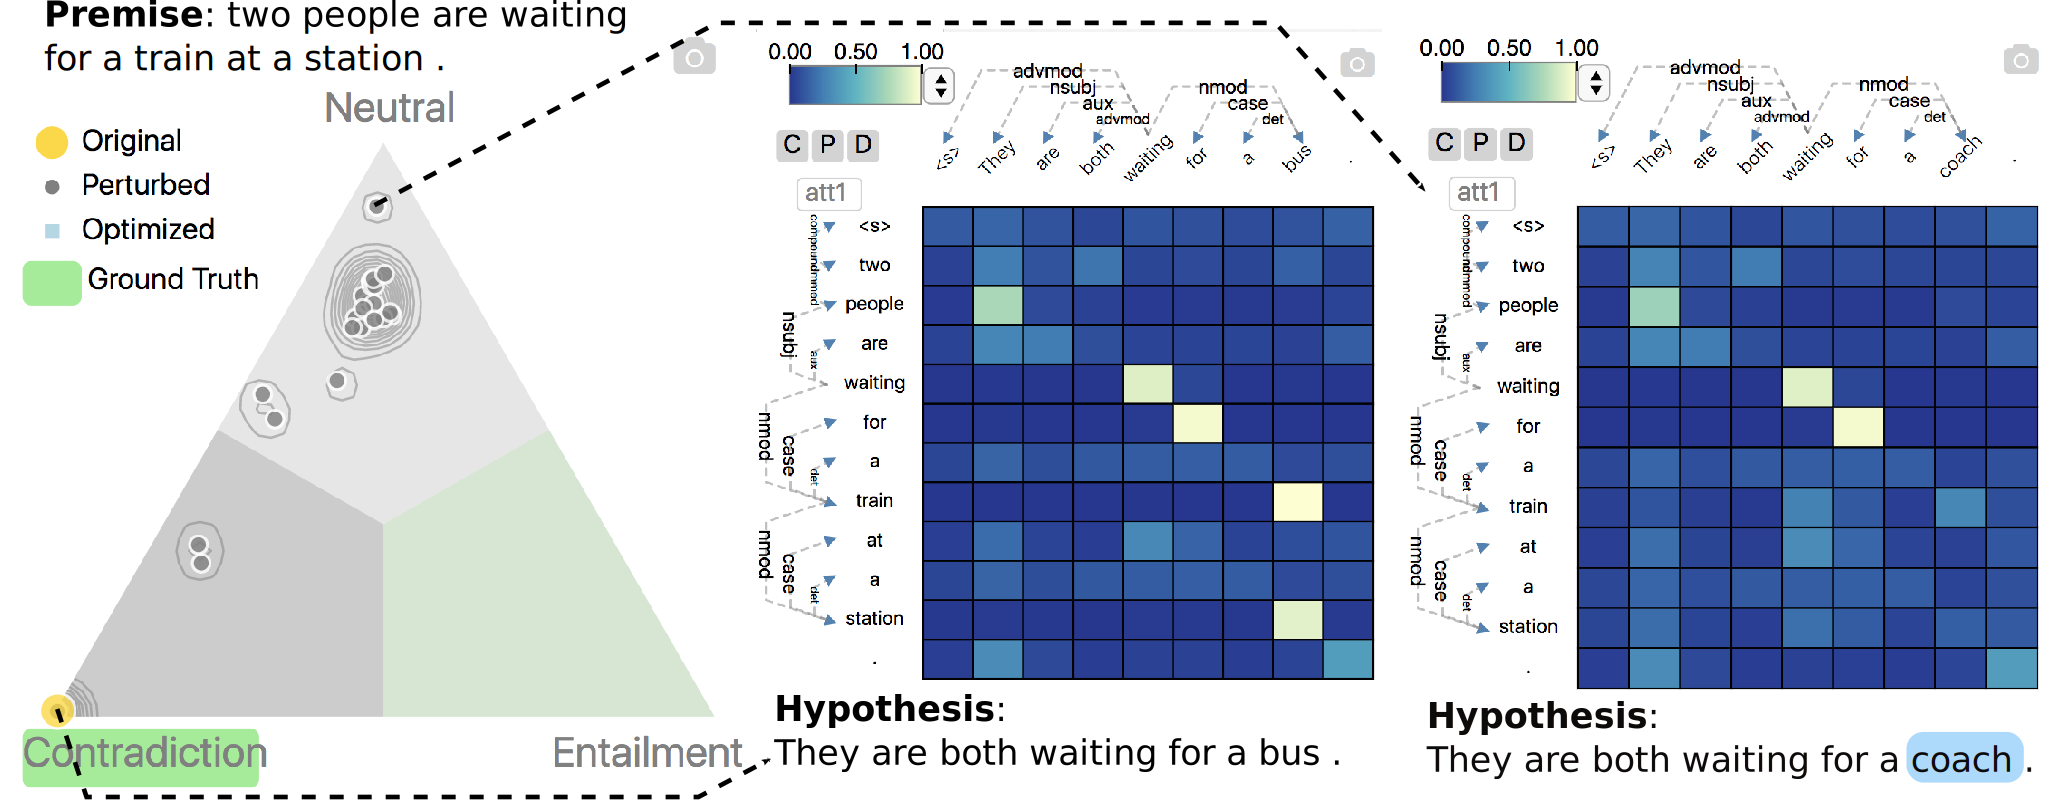
\includegraphics[width=0.9\linewidth]{failledEncoding}
 \caption{
The prediction is failed due to incorrect alignment. For all the failed case, 
 }
\label{fig:failedEncoding}
\end{figure*}


%One of the essential task for can be made in either of these stages.
% \shusen{difference in sensitivity among entail natural and contradict relationships}
% the generate the correct prediction for the wrong reason

Another
Does the model arrived at the correct prediction for the wrong reason?

\subsection{Scenario 2: What Does It Take to Correct a Wrong Prediction?}
In the previous section, we discussed how we can use forward prediction



\subsection{Scenario 4: Handcraft Example Analysis}
Well-known tough examples, such as the Facebook IPO example discussed in Section~\ref{sec:background}.

\subsection{Scenario 5: Explore Relationship Between Grammar and Attention}
Can attention capture grammar structure? Is 
%\subsection{Is the Prediction Stable?}
%\subsection{Where Are the Mistakes?}
%\subsection{How Attention Affect the Prediction?}
%\subsection{What Does It Take to Change the Prediction?}
%\subsection{Is Attention All You Need?}
